\subsection{Modalities}

\begin{figure}
    \centering
    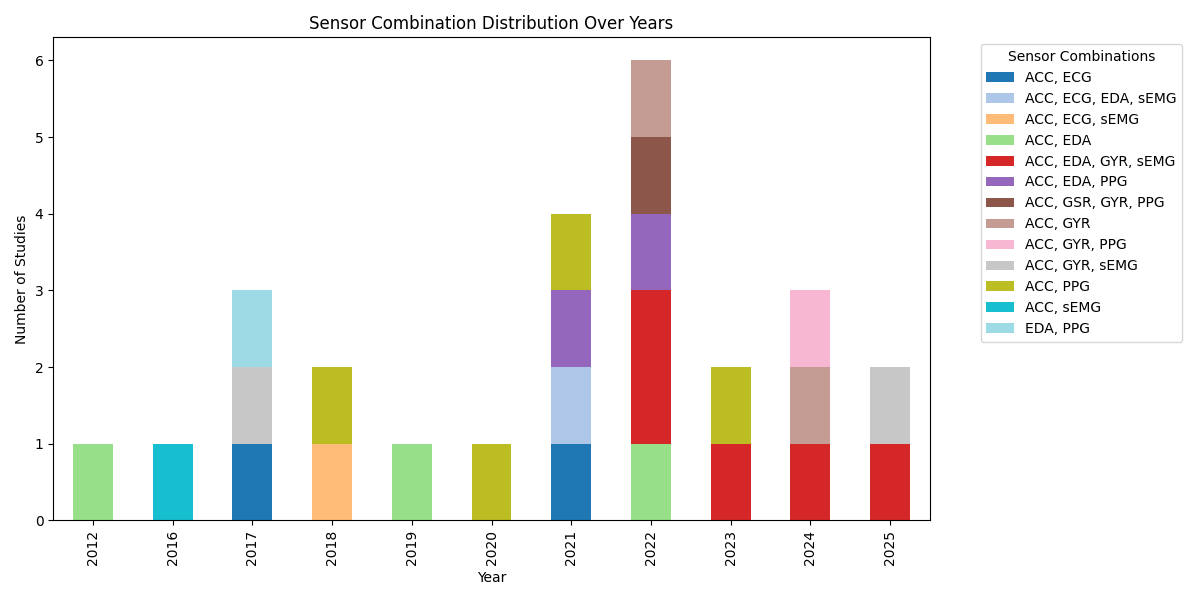
\includegraphics[width=1\textwidth]{Discussion/figures/Sensor_Combination_Distribution_Over_the_Years.png}
    \caption{Sensor combination distribution over the years.}
    \label{fig:sensor_comb_over_years}
\end{figure}

\subsubsection{Detection}
After reviewing all the included studies, it is apparent that non-EEG multimodal sensor configurations for detecting motor seizures are not only feasible but also show great promise compared to conventional detection and management methods. Several studies have assessed the performance of different combinations of sensor modalities and biomarkers, highlighting the importance of identifying the optimal configuration. However, to determine the best-performing combination of modalities and biomarkers, it is important to note that direct comparison across studies is challenging due to methodological heterogeneity, differences in study populations, and variability in training datasets.

Nevertheless, there has been a recent trend toward using the ACC + GYR + EDA + sEMG sensor combination (Figure \ref{fig:sensor_comb_over_years}). This combination performance is consistently high across studies (table no) despite different study setups. ACC + EDA is also one of the top performing combinations. This may be because these setups combine the reliability of motion-based detection through ACC, GYR, and sEMG with the stabilizing contribution of physiological signals such as EDA, which helps reduce false alarms and enhance overall performance. While this highlights the significance of EDA data in seizure detection, some studies have reported poor performance of EDA as a standalone modality and even when combined with other sensors such as PPG or ACC \cite{Yu2023-ss, Tang2021-td}. This variability across studies stems perhaps from the age-related variability in EDA signals reported by the pediatric study  \cite{Ge2023-ab}, highlighting the need for algorithms trained on EDA to count for such variability. 

Other physiological sensors such as PPG have also been widely used to extract biomarkers including HR \cite{Cogan2017-lg, Nasseri2021-xn, Vakilna2024-hk, Xu2022-tx, Arends2018-ew, Jiang2022-zu}, HRV \cite{Vakilna2024-hk, Jiang2022-zu}, SpO$_2$ \cite{Cogan2017-lg}, and BVP \cite{Nasseri2021-xn, Tang2021-td, Yu2023-ss}. Among these, BVP in particular has shown strong potential, consistently achieving high performance across seizure types.

ECG has also been employed to derive HR \cite{Van_Andel2017-yx, Hegarty-Craver2021-hk, De_Cooman2018-pq} and HRV \cite{Hegarty-Craver2021-hk}, with some studies reporting that unimodal ECG systems can achieve performance comparable to multimodal approaches \cite{De_Cooman2018-pq, Hegarty-Craver2021-hk}. However, ECG was used less frequently in the reviewed studies, largely due to its susceptibility to motion artifacts \cite{Van_Andel2017-yx} and the high inter-patient variability observed in cardiac-derived signals \cite{De_Cooman2018-pq, Van_Andel2017-yx}.

Because of these limitations, ECG has mostly been used in nocturnal studies \cite{Van_Andel2017-yx, De_Cooman2018-pq}. This is relevant since SUDEP is more likely to happen at night \cite{Friedman2022-mo}, and HR and HRV are under investigation as potential SUDEP biomarkers \cite{Barot2019-nx}. Thus, ECG may serve a dual role in seizure detection and monitoring SUDEP-related autonomic changes.

Some studies have also investigated the use of non-traditional biomarkers for seizure detection, and interestingly, several of these have demonstrated detection capabilities comparable to, or even exceeding, those of more established biomarkers. \cite{Hamlin2021-sd} investigated the incorporation of audio features  , derived from a MIC, in the detection system and reported that audio signals proved to be among the top ten features establishing separability between seizure and non-seizure data in four or five patients. \cite{Wang2025-ql} investigated the incorporation of attitude angle signals like PITCH or ROLL, which describe the orientation of the body/limb in the 3D space, in their detection system and reported that in multimodal combinations, adding PITCH or ROLL alongside or replacing ACC, GYR outperformed combinations that excluded them across all models. Instead of using raw ACC data, \cite{Xu2022-tx} used Number of Wrist Movements (NOWM), a derived feature that summarizes movement frequency over time windows, to distinguish seizure-like activity from normal daily movements.

Thus, future studies should validate the incorporation of these biomarkers into detection systems, while also assessing optimal sensor placement. Evidence from \cite{Milosevic2016-ee, De_Cooman2018-pq} shows that different sensor placements produce different outcomes, highlighting the importance of placement as a design consideration. In addition, studies should account for the variability exhibited by physiological signals across different populations by increasing and diversifying their cohorts, and by developing personalized models for highly patient-dependent modalities such as HR and HRV.

\subsubsection{Prediction and Forecasting}
Although the tasks and methodological scopes of the three studies varied, together they provide strong evidence for the feasibility of using wearable data from the Empatica E4 wristband in combination with machine learning or deep learning algorithms for seizure prediction and forecasting. Vieluf et al. \cite{Vieluf2023-ta, Vieluf2023-zv} demonstrated that the purely autonomic sensor set of EDA and PPG (from which HR and HRV are derived) could successfully discriminate pre-ictal periods in a substantial proportion of patients in their cohorts. However, the highest prediction performance was reported by Meisel et al. \cite{Meisel2020-ii}, where all available sensor modalities on the E4 device (EDA, PPG/BVP, ACC, and skin temperature) were incorporated into the forecasting models.